%%%%%%%%%%%%%%%%%%%%%%%%%%%%%%%%%%%%%%%%%%%%%%%%%%%%%%%%%%%%%%%%%%%%%%%%%%%%%%%%%%
\begin{frame}[fragile]\frametitle{}
\begin{center}
{\Large Quantum Machine Learning}
\end{center}
\end{frame}

%%%%%%%%%%%%%%%%%%%%%%%%%%%%%%%%%%%%%%%%%%%%%%%%%%%%%%%%%%%
 \begin{frame}[fragile]\frametitle{QML vs. traditional neural network/deep learning}
\begin{itemize}
\item  Similarities:
\begin{itemize}
\item  using “stacked layers” of transformations that make up a larger model
\item  data is used to inform updates to model parameters, typically to minimize some loss function
\end{itemize}

\item  Difference: QML models have access to the power of quantum mechanics and deep neural networks do not.
\item  Variational quantum circuits (QVC) is the QNN, has encoder circuit, the variational circuit and the measurement operators. 

\end{itemize}


\tiny{(Ref: My experience with TensorFlow Quantum,  Owen Lockwood, Rensselaer Polytechnic Institute)}

\end{frame}

%%%%%%%%%%%%%%%%%%%%%%%%%%%%%%%%%%%%%%%%%%%%%%%%%%%%%%%%%%%
 \begin{frame}[fragile]\frametitle{QVC}
\begin{itemize}
\item  The encoder circuit either takes naturally quantum data (i.e. a non-parametrized quantum circuit) or converts classical data into quantum data. 
\item  Variational circuit is defined by its learnable parameters. The parametrized part of the circuit is the part that is updated during the learning process. 
\item  Measurement operators extract information from the QVC some sort of quantum measurement (such as a Pauli X, Y, or Z basis measurements), a loss function (and gradients) is calculated on a classical computer and the parameters can be updated.

\item  QML can harness quantum phenomena, such as superposition and entanglement. 

\end{itemize}

	
\tiny{(Ref: My experience with TensorFlow Quantum,  Owen Lockwood, Rensselaer Polytechnic Institute)}

\end{frame}

%%%%%%%%%%%%%%%%%%%%%%%%%%%%%%%%%%%%%%%%%%%%%%%%%%%%%%%%%%%
 \begin{frame}[fragile]\frametitle{QVC}

\begin{center}
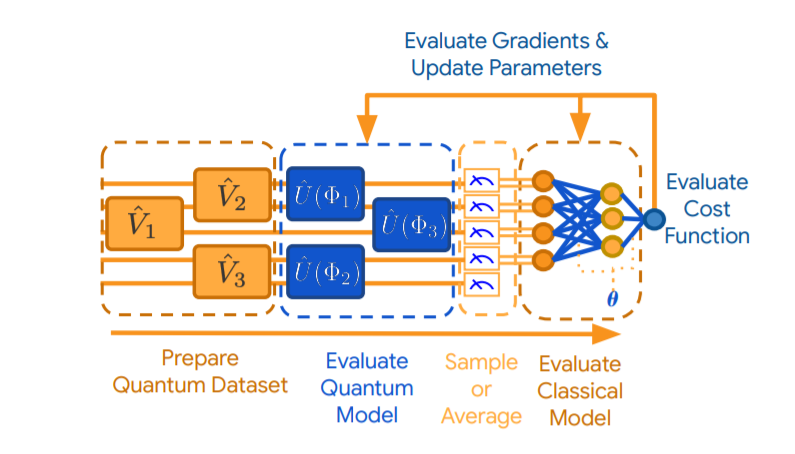
\includegraphics[width=\linewidth,keepaspectratio]{qvc}
\end{center}
	
\tiny{(Ref:My experience with TensorFlow Quantum,  Owen Lockwood, Rensselaer Polytechnic Institute)}

\end{frame}


%%%%%%%%%%%%%%%%%%%%%%%%%%%%%%%%%%%%%%%%%%%%%%%%%%%%%%%%%%%
 \begin{frame}[fragile]\frametitle{QVC}
\begin{itemize}
\item  Superposition stems from the wave function being a linear combination of multiple states and enables a qubit to represent two different states simultaneously (in a probabilistic manner). The ability to operate on these superpositions, i.e. operate on multiple states simultaneously, is integral to the power of quantum computing.
\item  Entanglement is a complex phenomenon that is induced via multi-qubit gates.
\item  Near term and current quantum devices have 10s-100s of quantum bits (qubits) like the Google sycamore processor. Because of their size and the noise, this hardware is often called Noisy Intermediate Scale Quantum (NISQ) technology.
\item  For classical ML researchers with experience in TensorFlow, TFQ makes it easy to transition and experiment with QML at small or large scales. The API of TFQ and the modules it provides (i.e. Keras-esque layers and differentiators) share design principles with TF and their similarities make for an easier programming transition.
\end{itemize}

	
\tiny{(Ref: My experience with TensorFlow Quantum,  Owen Lockwood, Rensselaer Polytechnic Institute)}

\end{frame}